\documentclass[11pt]{article}

\usepackage[table,xcdraw]{xcolor}
\usepackage{amssymb}
\usepackage[toc]{appendix}
\usepackage{mathtools}
\usepackage{amsmath} 
\usepackage[utf8]{inputenc}
\usepackage[czech]{babel}
\usepackage{url}
\usepackage{xcolor}
\usepackage[square,sort,comma,numbers]{natbib}
\usepackage{url}
\usepackage{pdfpages}
\usepackage{hyperref}
\usepackage{graphics}
\usepackage{pgfplots}
\hypersetup{
  colorlinks = true,
  citecolor = blue,
  urlcolor = blue,
  filecolor = red,
  linkcolor = gray,
}
\usepackage{algpseudocode, algorithm}
\usepackage[toc]{appendix}

\urlstyle{same}
\bibliographystyle{IEEEtran}

\addto\captionsczech{
  \renewcommand{\contentsname}{Table of contents}%
  \renewcommand{\figurename}{Figure}%
  \renewcommand{\tablename}{Table}%
  \renewcommand{\listfigurename}{List of figures}%
  \renewcommand{\listtablename}{List of tables}%
}
\title{Handling Missing Values in Decision Forests in the Encrypted Network Traffic}
\date{2018-05-25}
\author{Lukáš Sahula}

\begin{document}
  \begin{titlepage}
    \begin{center}
      \vspace*{1cm}

      \textbf{Handling Missing Values in Decision Forests in the Encrypted Network Traffic}

      \vspace{0.5cm}

      \textbf{Lukáš Sahula}
      \vspace{0.5cm}

      Bachelor's Thesis \\

      \vspace{2cm}

      
\includegraphics[scale=0.3]{thesis_res/ctu_logo_blue.pdf}

      \vspace{1cm}
      Department of Computer Science \\
      {\large Faculty of Electrical Engineering \\}
      {\LARGE Czech Technical University in Prague \\}

      \vspace{4.8cm}

    \end{center}

    \noindent Supervisor: Ing. Jan Brabec \\
    Program: Software engineering and technologies \\
    May 2018 \\
    
    
  \end{titlepage}
  \thispagestyle{empty}
  \newpage
  \thispagestyle{empty}
  \mbox{}
  \newpage
  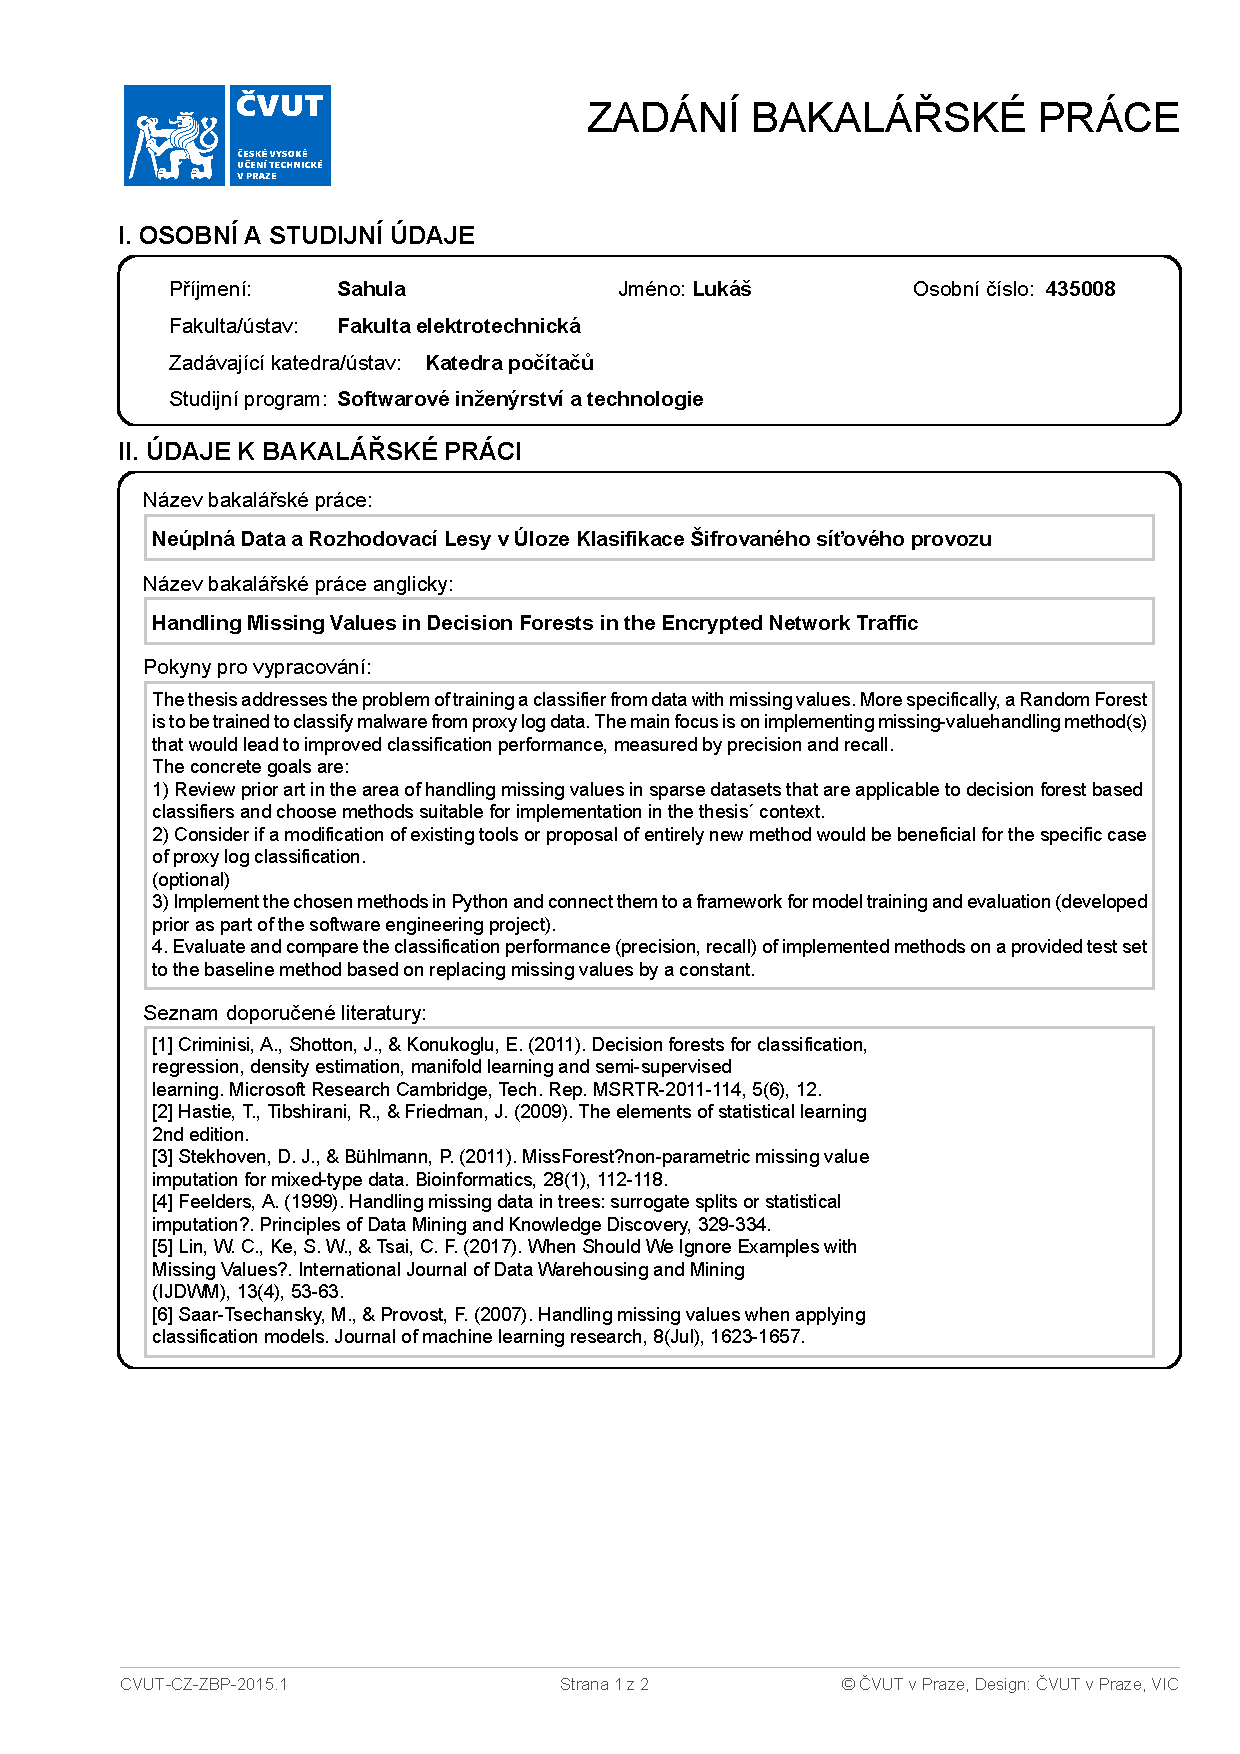
\includepdf[pages={1,2}]{thesis_res/zav_prace.pdf}
  \newpage
  \thispagestyle{empty}
  \mbox{}
  \newpage
  \section*{Acknowledgement}
    \thispagestyle{empty}
    First of all, I want to thank my supervisor Ing. Jan Brabec for his guidance, support, and for offering me such an interesting (and exhausting) topic while back in 2017 I did not know anything about machine learning and the only thing I was really interested in was to find something "cool"{ }to do with the Python programming language.
    \\~\\
    I also want to give my thanks to my family for their support and the trust they put in me. Especially to my brother Peter for regularly putting things in perspective.
    \\~\\
    An immeasurable amount of thanks also goes to my friend Tomáš, for he was ready to explain and talk about anything even remotely related to mathematics at all times.
  \newpage
  \section*{Declaration}
    \thispagestyle{empty}
    I declare that the presented work was developed independently and that I have listed all sources of information used within it in accordance with the methodical instructions for observing the ethical principles in the preparation of university theses.
    \\~\\
    ..................... in Prague, on the 25th of May 2018
  \newpage
  \section*{Abstract}
    \thispagestyle{empty}
    This thesis examines the problem of malware classification using the random forest classifier trained on network traffic dataset. The dataset contains hundreds of millions of labeled objects, some of which are related to malware infection. However, roughly half of the datasets values are missing and these missing values have to be handled before or during the process of classification. The thesis discusses a number of existing approaches to missing data imputation and compares the results of those that are relevant to datasets of this scale. Furthermore, this work provides an analysis of the dataset itself in order to find the correlations between pairs of features and their missingness.
    \\~\\
    {\bf Keywords:} malware, classification, random forests, supervised learning, missing values, imputation, feature, correlation 
    \\~\\
    Tato práce zkoumá problém klasifikace malware za použití klasifikátoru náhodných lesů trénovaných na datasetu získaném ze síťového provozu. Tento dataset obsahuje stovky milionů kategorizovaných záznamů, z nichž některé jsou spojené s určitým druhem malwarové infekce. Avšak zhruba polovina hodnot v datasetu chybí a s těmito chybějícími hodnotami je nutno se vypořádat, ať už před procesem klasifikace, nebo během něj. Práce ukáže několik existujících způsobů imputace chybějících dat a porovná výsledky těch, které jsou vhodné k použití s datasetem těchto rozměrů. Dále práce poskytne analýzu použitých dat se záměrem nalezení míry korelace mezi páry jednotlivých atributů a toho, za jakých podmínek jednotlivé atributy chybí.
    \\~\\
    {\bf Klíčová slova:} malware, klasifikace, náhodné lesy, učení s učitelem, chybějící hodnoty, imputace, feature, korelace
  \newpage
  {\hypersetup{hidelinks}
  \thispagestyle{empty}
  \tableofcontents
  \thispagestyle{empty}
  \newpage
  \thispagestyle{empty}
  \listoffigures
  \listoftables}
  \newpage

  \section*{Introduction}
  \addcontentsline{toc}{section}{Introduction}
    Machine learning and cybersecurity are two highly significant subjects of today's tech industry. With machine learning being utilized in various fields at an increasing rate, it is no wonder that it has found its uses even in the field of cybersecurity. This thesis touches both of these subjects in the context of automated {\it malware classification}, with the main focus being dealing with {\it missing values} using the {\it random forest classifier}.
    \\~\\
    In order for a classification algorithm to work, it has to be trained on some set of data. In this case the datasets are encrypted network traffic and as such they contain a moderate amount of {\it missing data}. Missing data, also referred to as missing values mark the absence of a value somewhere inside the dataset. Most classification algorithms are not designed with an implicit way of dealing with missing values and thus they have to be handled before or during the classification process.
    \\~\\
    Over the past two decades \cite{otfi}\cite{lwd}\cite{mia}, a moderate amount of methods for dealing with missing data has been introduced, but none has yet shown superior results that would put it above the others. Plenty of methods are somewhat situational and work only with specific cases of missing data. Thus it is not clear which method to choose at which time. This thesis studies these methods along with analysing the network traffic datasets in order to find out the most efficient one.
    \\~\\
    The dataset used in this thesis contains real and huge data spanning across more than a hundred of enterprises. As such, one of the concerns in choosing the methods for handling missing data are its computational speed and memory demands.
    \\~\\
    The thesis consists of several sections. At the beginning, there is a brief introduction to malware classification, followed by an explanation of the classification algorithm often connected to the missing data problem - the {\it random forest classifier}. The next chapter provides an analysis of the network datasets. The chapter after that concerns itself with missing data mechanisms and gives a summary of known algorithms for missing data {\it imputation}. The last section is dedicated to the conducted experiments and results of this thesis.
  \newpage
  \section{Malware and classification}
      This chapter serves both as a general introduction to the term {\it malware} and as an introduction to {\it machine learning}, specifically to one of its subsets, {\it classification}. After explaining both terms, there is a short section dedicated to connecting the two terms.
    \subsection{Malware}
      {\it Malware} is an abbreviated form of the term malicious software. It is often used when referring to viruses, spyware, ransomware, and other software designed to cause harm to a computer, server, network or a mobile device. \cite{malware}
      \\~\\
      Viruses are computer programs with the goal of spreading from one file to another across one or multiple devices through a network undetected and without consent of the user. A common misinterpretation of viruses is that they are programs designed to delete or move data, however, this damage is often a side effect. The definition of a virus is that it spreads itself. \cite{malware}
      \\~\\
      Spyware is a form of computer program that runs on the infected computer and tracks its user's habits to form a pattern that can be then used for advertisements or sent to the spyware's creator. \cite{malware}
      \\~\\
      Ransomware is a potentialy very dangerous software that threatens to delete, block or publish the target's data if the program's author's requirements are not met. \cite{ransomware}
      \\~\\
      When malware spreads through the network, or when it communicates with their command and control servers, it leaves a detectable trace in the network traffic. What more, these traces can often be found much sooner (ranging from weeks to months) than researchers are able to capture a sample of the invading malware. \cite{network} This only emphasizes the importance of utilizing machine learning in the context of malware detection, manual systems and blacklists are not enough today.
      \\~\\
      According to the five years long study by Georgia Institute of Technology, the endpoints with which specific malware communicates do not change in long time periods (years). This means that once a node in the network suspicious of being infected is found, it is possible to look for traffic going in and out, which in turn can help with identifying other infected devices. \cite{network}
    \subsection{Classification}
      In statistics and machine learning, classification is the process of assigning a specific category, or a {\it class}, to which a new object or an observation belongs. \cite{elements} This assignment, or {\it prediction}, is done after processing a set of previously categorized data, often called the {\it training dataset}. \cite{elements} This is done by a classification algorithm, known as a {\it classifier}. \cite{elements} This classifier learns from a set of data, for example emails labeled as spam or non-spam, in order to predict the category of new incoming emails. That way an email client can move unwanted spam to the spam folder and keep the relevant mail in the inbox. Another is predicting whether a patient's tumor is benign or malign, based on the hospital records with data from other patients. Or, as will be the case in this thesis, whether an instance of network traffic is the related to (and which) malware, based on data gained from network proxy logs.
      \\~\\
      Within the terminology of machine learning, classification is in the category of {\it supervised learning}. \cite{mlintro} Supervised learning means that the classifier learns from the training dataset with labeled data. This dataset is often processed into the form of a matrix $\mathbf{X}$ in order to make the work with it more convenient. The rows in this matrix contain the observed attributes, called {\it features}, of each individual object. The rows are sometimes called {\it feature vectors}, labeled $\mathbf{x} = \left( x_1, x_2, x_3, ..., x_i \right)$ where $i$ denotes the number of features. Feature vector sometimes refers to the column, containing all values of a single feature across all objects. However, in this thesis, feature vectors refer to the rows. These features are quantifiable and can be categorical (smoker or non-smoker), integer-valued (age of the patient in years), or real-valued (patient's body temperature). Since the learning is supervised, the dataset also includes a column with the class labels of each observed object labeled $\mathbf{Y}$.
      \\~\\
      When the classifier is trained, it can predict the classes of new objects based on their features. The mathematical function implemented by the classifier maps input feature vectors $\mathbf{x}$ of a matrix $\mathbf{X}$ to a class $\mathbf{c}$ from the set of classes $\mathbf{C}$. The performance of the classifier is usually tested on another set of data called the {\it testing dataset}. That is done to avoid {\it overfitting} - "the production of an analysis that corresponds too closely or exactly to a particular set of data, and may therefore fail to fit additional data or predict future observations reliably". \cite{oxford} According to this definition, an overfitted classifier could be able to predict the classes of the objects in its training dataset accurately, yet completely miss the classes of new objects. The opposite of overfitting is {\it underfitting}, which can also be avoided by measuring the classifier's performance on the testing dataset. In machine learning, overfitting and underfitting is sometimes also called "overtraining" and "undertraining" respectively.
      \\~\\
      Classification does not always have to be binary, meaning the data can be of more than two categories. This is called {\it multiclass classification}. Returning to the example of e-mail classification, some classifiers could be trained to predict whether an incoming e-mail belongs to {\it work}, {\it school}, or {\it personal} categories.
      \\~\\
      There are also other forms of classification, like the {\it multilabel classification}. In multilabel classification, multiple classes can be assigned to an observation. This makes sense in cases where the categories are not mutually exclusive. However, this thesis will be focusing only on the problem of multiclass classification.
    \subsection{Malware classification}
      As was mentioned in the malware section of this chapter, malware can often be detected very early by monitoring the incoming and outgoing network traffic of the observed device. However, this is not something that every computer user can do, and even then it can prove to be a relatively tedious task. In this day and age there can be thousands of individual network requests performed by a computer and going through them manually is impossible. As such, the reasonable thing to do would be to take all the data and feed it to a machine learning algorithm to do the work instead. Another point to be made is that current solutions such as static rules defined by domain or server blacklists do not work very well as they do not work dynamically and new entries have to be added manually.
      \\~\\
      This thesis is based on the work done on labeled network datasets containing observations of more than two hundred different classes of malware. The goal is not only to be able to predict whether a computer is infected with malware, but also to decide which class of malware infection it is. It is, therefore, a case of multiclass classification.
      
  \newpage
  \section{Random forest classifier}
    {\it Random forests} or {\it random forest classifiers} are the central focus of this thesis because they are most suited for the malware classification problem. They can handle {\it multiclass classification}, evaluate data relatively fast and they are not heavily affected by {\it imbalanced datasets}. \cite{brabec} They run efficiently on large amounts of data and give estimates of what feature variables are important for classification. \cite{breiman}
    \\~\\
    This chapter explains in detail how random forests work and how they can be implemented. As the name implies, random forest is an ensemble of learning algorithms called {\it decision trees}. In order to understand random forests, decision trees are the first thing that needs to be explained.
    \subsection{Decision trees}
      \subsubsection{Overview}
        {\it Decision tree classifier} is a classification algorithm named because of its structure resembling a tree known from graph theory. Another variation of a decision tree is the regression tree, which only differs in that the predicted outcome is not a class but a real value. One of the most significant publications about decision trees is {\it Classification and Regression Trees} by L. Breiman. It introduces the {\it CART algorithm} for growing both classification and regression trees. \cite{cart} Other algorithms for growing decision trees also exist, for example the {\it ID3 algorithm} or the {\it C4.5 algorithm}.
        \\~\\
        Prediction using a decision tree can be interpreted as a set of questions asking about the attributes of the observed object. For example, predicting whether a picture is taken outdoors or indoors could work as follows:
        \begin{itemize}
          \item Is the top of the picture blue?
          \begin{itemize}
            \item If yes, the picture was taken outdoors.
            \item If no, is the bottom of the picture green?
            \begin{itemize}
              \item If yes, the picture was taken outdoors.
              \item If no, the picture was taken indoors.
            \end{itemize}
          \end{itemize}
        \end{itemize}
        As can be seen in the example, a grown tree is built from a root node, decision nodes and terminal nodes, also called {\it leaves}. All leaves are associated with the resulting prediction class. Each decision node contains information about its split, which consists of the selected feature and its value. When an observed object is analysed to predict its class, the value of the feature in question is compared with the value stored at the decision node. Depending on the result of this comparison, the object is then sent to the left child or the right child of the node. When the object reaches a leaf node, it is given the class that is associated with it. This explanation is visualised in Figure [\ref{figure:decision_tree}].
        \begin{figure}
          \centering
          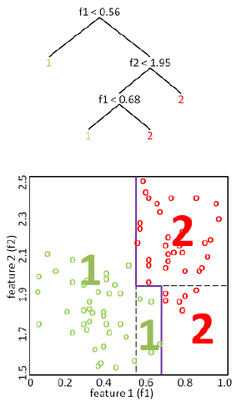
\includegraphics[scale=0.7]{thesis_res/decision_tree.png}
          \caption{Picture of a decision tree with the training data used for its growth \cite{digstaining}}
          \label{figure:decision_tree}
        \end{figure}
      \subsubsection{Strengths}
        In comparison with other classification algorithms, decision trees have various strengths and advantages, like:
        \begin{itemize}
        \item They require little data preparation, for example data normalisation is not needed like in other techniques. \cite{isl}
        \item They work with both numerical and categorical data. \cite{isl}
        \item They perform well with large datasets within reasonable time. \cite{breiman}
        \item They are easily interpretable by most people after a brief explanation. The graphical representation of the tree is also very easy to follow and the decision making process is similar to how people generally make decisions in real life. \cite{isl}
        \end{itemize}
      \subsubsection{Weaknesses}
        However, decision trees are not perfect as classifiers go because they also have some weaknesses, for example:
        \begin{itemize}
        \item They are not as accurate as other approaches. \cite{isl}
        \item They are not very robust, a small change in training data can lead to a big change in the decision tree, leading to different results. This is called {\it overfitting}. \cite{isl}
        \end{itemize}
        All these disadvantages are going to be addresed again in the random forests part of this chapter.
      \subsubsection{Growing a decision tree}
        Training a decision tree classifier is done by recursively partitioning the input data according to the best calculated split. The split specifies the feature and value at which the data is partitioned into two parts. Once the data is partitioned, a new node $t_i$ is created and the process continues at its children, see algorithm [\ref{alg:grow_tree}]. If it is for some reasons impossible or not needed to split the input dataset, a leaf node is created and the recursion does not continue. \cite{brabec}
        \\~\\
        To expand on the notation, the nodes are numbered in breadth-first order, starting with the root node $t_0$. Since all the trees encountered in this thesis are binary, the left child of node $t_i$ can be denoted as $t_i^L$ and the right child can be denoted as $t_i^R$. Since the dataset is being recursively partitioned, the subset of samples belonging to node $t_i$ can be denoted as $S_i$. The subset of samples belonging to the left child of node $t_i$ is denoted as $S_i^L$ and the one belonging to the right child as $S_i^R$. It follows that $S_i = S_i^L \cup S_i^R$ and that $S_i^L \cap S_i^R = \theta$ for every inner node. \cite{brabec}
        \\~\\
        \begin{algorithm}
          \caption{This algorithm shows how the decision tree classifier is grown recursively. It uses the dataset $S_i$ as the input and returns the root node $t_0$ of the tree. \cite{brabec}}
          \label{alg:grow_tree}
          \begin{algorithmic}[1] % The number tells where the line numbering should start
            \Function{GrowTree}{$S_i$}
              \If{$ShouldCreateLeafNode(S_i)$}
                \State \Return $CreateLeafNode(S_i)$
              \EndIf
              \State $\theta \gets FindBestSplitParameters(S_i)$
              \State $S_i^L, S_i^R \gets SplitDataset(S_i, \theta)$
              \State $t_i^L \gets GrowTree(S_i^L)$
              \State $t_i^R \gets GrowTree(S_i^R)$
              \State \Return $t_i$
            \EndFunction
          \end{algorithmic}
        \end{algorithm}
      \subsubsection{When to create a leaf node}
        Multiple conditions are checked before the dataset $\mathbf{S_i}$ is split, depending upon which the split may not even take place and a leaf node gets created. The conditions may differ among different implementations of the tree. The ones used for the purposes of this thesis are the following:
        \begin{itemize}
          \item Check the number of unique classes in dataset $\mathbf{S_i}$. If all the samples are of the same class, there is no need to split further and a leaf node can be created. \cite{brabec}
          \item Check if it is possible to split the dataset $\mathbf{S_i}$ at least once. It is possible, that all the feature vectors in $\mathbf{S_i}$ are the same, but their classes differ. If that is the case, a leaf node is created. \cite{brabec}
          \item One of the hyperparameters of a decision tree is usually the minimum number of samples required to split the dataset ($minSamplesToSplit$). If $|\mathbf{S_i}| < minSamplesToSplit$ then a leaf node is created. This parameter is often set low in random forests because it allows the trees to grow deeper. \cite{brabec}
        \end{itemize}
        Other implementations also include the $maxDepth$ hyperparameter, limiting the maximum depth of a tree, or the change in {\it impurity measure} (information gain) as the stopping condition during node splitting. \cite{brabec}
      \subsubsection{How to create a leaf node}
        The leaf node contains the subset of sampled associated with it. Upon arriving in a leaf node during prediction, the most common choice is to return the class with maximum frequency in the samples. Different implementations can return the whole normalized histogram of classes in the samples, where each value represents the probability of the object belonging to the given class.
      \subsubsection{Finding the best split}
        \label{sec:split}
        The best split out of all possible splits of the dataset is defined as the one that provides the largest {\it information gain}. Information gain corresponds to the decrease in impurity in the node's children. {\it Impurity measure} of node's subset $\mathbf{S_i}$ is a function $i(\mathbf{S_i}) \in \mathbb{R}$. The purer the data (the lower the impurity measure), the more confidence can be given in the node's prediction. Therefore, the split $\theta_i$ that reduces the impurity in the node's children the most, is also the best split. To find it, all possible splits have to evaluated. The decrease in impurity is defined as follows:
        \begin{equation}
          \Delta i(\mathbf{S_i}, \theta_i) = i(\mathbf{S_i}) - \frac{|\mathbf{S_i^L}|i(\mathbf{S_i^L}) + |\mathbf{S_i^R}|i(\mathbf{S_i^R})}{|\mathbf{S_i}|}
        \end{equation}
        There are several impurity measures, most common of which are {\it Gini impurity} and {\it entropy}. Studies show that there is not a significant difference between the two and therefore can be used interchangebly. \cite{gini} Only entropy is used for the purposes of this thesis. Entropy is defined as:
        \begin{equation}
          H(\mathbf{X}) = - \sum_{c \in \mathbf{C}}^{n} p(c)\log{p(c)}
        \end{equation}
        Where $\mathbf{C}$ is the set of classes and $p(c)$ is the frequency of class $c$ in the node's subset $\mathbf{S_i}$. \cite{brabec} If the class is not in the subset at all, it does not add to the sum anything either. The entropy is at its maximum if the classes in the subset $\mathbf{S_i}$ are equally distributed. If all the objects belong to the same class, the entropy equals to zero. As was stated earlier, information gain corresponds to the decrease in impurity $\Delta i(\mathbf{S_i}, \theta_i)$. \cite{brabec}
        \\~\\
        To select the best split, all splits along every dimension have to be evaluated. \cite{brabec}. This can be optimised, as is shown in algorithm [\ref{alg:best_split}]. The data points are grouped together to reduce duplicities. This means that out of 50 objects having the same coordinate in the evaluated dimension, we only remember the class counts of those 50 objects and the coordinate itself. Further work in finding the split is done only with the class counts. \cite{brabec}
        \begin{algorithm}
          \caption{This algorithm shows how to find the split with the highest information gain. \cite{brabec}}
          \label{alg:best_split}
          \begin{algorithmic}[1] % The number tells where the line numbering should start
            \Function{FindBestSplitParameters}{$S_i$}
              \State $maxGain_\Delta \gets -\infty$
              \For{$all dimensions$}
                \State $counts^L \gets (0, 0, ..., 0)$
                \State $counts^R \gets GetClassCounts(S_i)$
                \State $coordinates \gets$ find unique coordinates in dimension
                \State $Sort(coordinates)$
                \For{$point \in coordinates$}
                  \State $counts^L \gets$ add class counts present on point
                  \State $counts^R \gets$ remove class counts present on point
                  \State $currentGain_\Delta = ComputeGain_\Delta(counts^L, counts^R)$
                  \If{$currentGain_\Delta > maxGain_\Delta$}
                    \State $maxGain_\Delta \gets currentGain_\Delta$
                    \State $\theta_i \gets$ create split parameters from point and neighbor
                  \EndIf
                \EndFor
              \EndFor
              \State \Return $\theta_i$
            \EndFunction
            \Function{$ComputeGain_\Delta$}{$counts^L, counts^R$}
              \State $size^L \gets Sum(counts^L)$
              \State $size^R \gets Sum(counts^R)$
              \State \Return $- \frac{size^L \times H(counts^L) + size^R \times H(counts^R)}{size^L + size^R}$
            \EndFunction
          \end{algorithmic}
        \end{algorithm}
        Since many features can have only a very limited set of values, this optimisation can give a significant performance boost to the algorithm. \cite{brabec} By sorting the coordinates, the class counts can be added to $counts^L$ and removed from $counts^R$ in an organised way. That is done by iterating over all of the sorted coordinates throughout the dimension. This approach also makes the time of each entropy calculation constant because it is dependent only on the number of classes, instead of the number of objects. \cite{brabec}
        \\~\\
        After finding the best possible split $\theta_i$, the dataset $\mathbf{S_i}$ is then partitioned into $\mathbf{S_i^L}$ and $\mathbf{S_i^R}$ by a threshold set by the splits feature and value. Considering the number of dimensions and classes are constant, the worst case time complexity of this algorithm is $\mathcal{O}(|\mathbf{S_i}|\log{\mathbf{S_i}})$. The worst case is the one where there are no data points with duplicate coordinates and the sorting of the coordinates will equal to sorting the whole dataset. In practice, however, it can be expected that the performance will be better, but still highly dependant on the given data. \cite{brabec}
    \subsection{Random forests}
      Since single decision forests tend to overfit to the training data \cite{isl}, are not making very accurate predictions, and tend to change significantly with small alterations to the datasets, they do not look very good compared to other approaches. However, an {\it ensemble method} called random forests deals with these issues. It groups multiple randomized decision trees together and builds a much stronger classifier. There are two categories of ensemble methods, {\bf boosting methods} and {\bf averaging methods}. Boosting methods create the weak classifiers sequentially and every classifier is an improvement of the previous one. \cite{brabec} Boosting methods are not in the scope of this thesis, so only averaging methods are going to be discussed.
      \\~\\
      Averaging methods build the classifiers in parallel and average their predictions. This averaging decreases the potentially high variance of the weak classifiers. Random forests belong to this category. \cite{brabec} Depending on the implementation, the predictions are aggregated either by {\it majority voting} or by {\it soft voting}. Majority voting chooses the most frequent class among the predictions of all the trees, while soft voting averages the class probability results from each tree. \cite{ensemble} For random forests to bring an improvement over decision trees, each tree in the forest has to be different. This is where the "random" in the name comes from. Randomness is injected into each tree in different ways, depending on the implementation. It is usually done by introducing randomness to the node splitting process, or by selecting a random subsample from the training dataset. \cite{brabec} {\it Breiman forests} \cite{breiman}, by far the most commonly used random forest algorithm, combine {\it bootstrap aggregating} and {\it random feature subsets} at each node to inject randomness into the forest. This is done in this thesis as well.
      \subsubsection{Bootstrap aggregating}
        Bootstrap aggregating, also called {\it bagging}, was first introduced in \cite{bagging}. For a forest of size $m$ and training dataset of size $n$, bagging assigns a dataset of size $n'$ to each of the $m$ trees. These datasets are created by selecting random samples with replacement from the training dataset. This means that some objects are not present in the sampled dataset and some objects might be repeated. The trees are then trained on their corresponding sample. The size of the bootstrapped datasets is usually parametrized in the forest, but the most common choice is to select $n'$ = $n$.
      \subsubsection{Random feature subsets}
        Random feature subsets inject randomness directly into the growing process of the decision tree. When looking for the best possible split, a standard decision tree looks across all dimensions of the training data. [\ref{alg:best_split}] However, trees in Breiman forests only use a random subset of the dimensions, sampled for each split node individually. The number of dimensions selected by this sampling is another hyperparameter of the random forest, denoted in this thesis as $maxFeatures$. The value of this parameter affects the correlation between individual trees. \cite{brabec} The least corellation would be achieved by setting $maxFeatures = 1$. Selecting $maxFeatures = numberOfDimensions$ removes all randomness from the individual trees' splitting process, leaving only the randomness induced by bagging. That, however, is usually not enough. More so when the training dataset contains a big amount of objects. In this particular case, the forest would not bring many advantages over a decision tree. An empirically tested rule of thumb says that $splitFeaturesCount = \sqrt{numberOfDimensions}$ is a reasonable default for classification tasks. \cite{ert} Curiously enough, the default for regression classes seems to be equal to the number of dimensions. \cite{ert}
  \newpage
  \section{Network dataset}
    \label{sec:datadesc}
    This chapter centers on the network datasets used for malware classification. The following subsections provide a description of the dataset as well as an analysis done to gather more information on the correlation among pairs of features. The last part of this chapter tries to answer why most of the studied algorithms do not provide satisfying results.
    \subsection{Dataset description}
      The data comes from network traffic of more than a hundred large enterprises taken on five days of early 2017. The dataset contains roughly 600 million of individual records. Out of these, only 4 million are labeled as positive, making the dataset heavily imbalanced. Imbalanced dataset means that "at least one of the classes constitutes only a very small minority of the data." \cite{imbalanced} In this case, each of the positive classes are a minority while the negative class is an overwhelming (more than 99\%) majority. However, a random sampling of the negative objects was done in order to allow faster computation, which also deals with this issue. Out of all the negative objects, only 1.5 million of objects was sampled to make the proportion between classes more balanced.
      \\~\\
      Each object in the dataset consists of 55 columns. The first column represents the class to which the object belongs. The next 3 columns contain metadata information of the object and are not used for training and prediction. Those are the timestamp, user and host and they are used in aggregated evaluation of the classifier, described later in Chapter [\ref{sec:experiments}]. The remaining 51 columns are the features. Because of the sensitivity of the data, we are unable to publish their exact meaning. However, some examples of the features could be the number of bytes transmitted or received, duration of the network event, direction of the packet, the amount of incoming and outgoing packets, the IP address of the destination, etc. The data comes from three different sources. One of them is the network flow, one is the output of {\it Cisco CTA} engine, which detects the periodicity of connections as an example. The third source is computed globally, for instance the number of users connecting to the server or the information from DNS. The individual values of these features are represented by integers and real numbers.
      \\~\\
      The objects in the dataset all come from a set of 115 classes in total.
      \\~\\
      An important thing that needs to be taken into consideration when working with a dataset like this is the fact that the samples are taken from various days. This could potentially mean that a classifier can perform better on data taken from the same day or from the day after, but worse with data from the next month, or even a year. The samples analysed in this thesis are from days week apart in January, with one day from the beginning of March. In this small scale, however, no significant differences in performance that could be attributed to this were found.
    \subsection{Analysis}
        \label{sec:analysis}
        This subchapter examines the dataset and attempts to analyse the nature of missingness of its missing data. The first step of the analysis was to look at the features and see how often and when are they missing. After that, a {\it correlation matrix} was constructed to see the correlation among pairs of the features. Another correlation matrix was constructed from an altered dataset where each value was replaced by 1 and each missing value was replaced by 0 to see the how correlated the features' missingness is. A matrix of conditional probabilities was also created to provide information on how often is one feature not missing when the other one is missing.
      \subsubsection{Missingness}
        In the whole dataset, there are only 4 features that are not missing from any of the objects. 12 features, on the other hand, are missing in more than 90\% of the time. The average missingness throughout the dataset is roughly 51\%. Some features are closely tied together and when one of them is missing, the others are missing as well. Therefore the assumption is that some of the features are not missing at random. [\ref{sec:missmech}] Other features, however, do not fulfill this assumption and could possibly be used when others are missing if they are somehow correlated.
      \subsubsection{Correlation matrix}
        The second step in this analysis was to figure out how are the features correlated to each other. For that, the {\it Pearson correlation coefficient} was used, defined as: \cite{correlation}
        \begin{equation}
          \rho_{X, Y} = \frac{cov(X, Y)}{\sigma_X \sigma_Y}
        \end{equation}
        In this equation $X$ and $Y$ are features and the result is the amount of correlation between them. Correlation is bound between -1 and 1: \cite{correlation}
        \begin{equation}
          -1 \leq \rho_{X, Y} \leq 1
        \end{equation}
        The closer the correlation is to 1, the stronger the positive linear dependence between the features is and vice versa, the closer the correlation is to -1, the stronger the negative linear dependence between the features is. For the purposes of this thesis it is not required to differentiate between positive and negative correlation because both are equally important. Therefore an absolute value of correlation is used in the following analysis.
        \\~\\
        Computing this correlation for each existing pair of all the features in the dataset we get a 51 x 51 symmetric matrix with the number 1 on the main diagonal. Every element in this matrix symbolizes the correlation between the feature represented by the element's row, and the feature represented by the element's column. The matrix is symmetric because the pair of features (X, Y) has the same correlation as the pair (Y, X). Furthermore, the main diagonal is full of 1s because a feature is completely correlated with itself. However, in some cases it is impossible to compute the correlation, and that is when the feature is always missing. In this thesis, its correlation value is replaced by 0. With this matrix, it is possible to create a heatmap in order to provide a more visual representation, seen in Figure [\ref{figure:correlation_matrix}]. It is possible to see that some pairs of features in fact are highly correlated.
        \begin{figure}
          \centering
          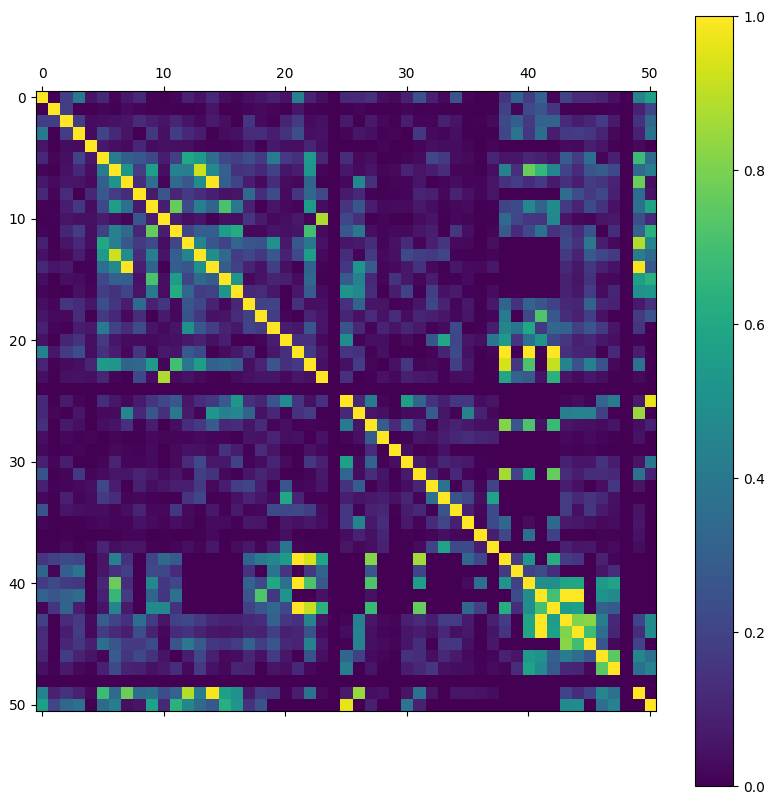
\includegraphics[scale=0.4]{thesis_res/corr/heatmap_cropped.png}
          \caption{Correlation matrix showing the amount of correlation among pairs of features}
          \label{figure:correlation_matrix}
        \end{figure}
      \newpage
      \subsubsection{Missingness correlation matrix}
        The same way as before, it is possible to create a correlation matrix from the dataset where every not missing feature is replaced by number 1 and every missing feature is replaced by number 0. This correlation matrix tells us how correlated the missingness of pairs of features is. To put it in other words, it shows how dependent the fact that a feature is missing on another feature being missing or not missing. A heatmap of this matrix is in Figure [\ref{figure:missingness_matrix}]. However, the features that are never missing, or the ones that are always missing, have no variance because their value is either always 1 or always 0. Their correlation therefore could not be computed and set to 0. It is possible to see that the most correlated are the features that are next to each other, meaning that they come from the same source or that they are connected to each other. This ties together with the assumption that those features are not missing at random [\ref{sec:missmech}].
        \begin{figure}
          \centering
          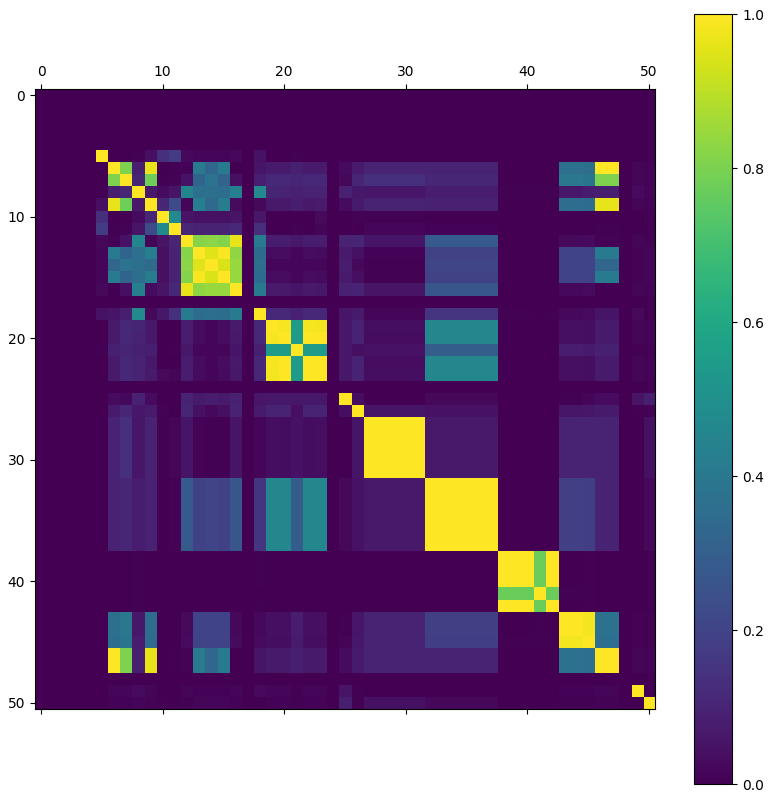
\includegraphics[scale=0.4]{thesis_res/miss/heatmap_cropped.png}
          \caption{Correlation matrix showing the amount of correlation among pairs of features based on them being missing or not}
          \label{figure:missingness_matrix}
        \end{figure}
      \newpage
      \subsubsection{Conditional probabilities matrix}
        The conditional probabilities matrix represents the probability that feature X is not missing when feature Y is missing [\ref{eq:prob}]. This matrix is not symmetric because the probabilities differ for pairs (X, Y) and (Y, X). [\ref{figure:cond_prob_matrix}] The yellow belt going from the top to bottom symbolizes the features there are never missing.  The probability that the first four features are missing is zero, therefore the conditional probability that other features are not missing when the first four are is also zero. The value on the i-th row in the j-th column gives the probability that feature j is not missing when feature i is missing.
        \begin{equation}
          \label{eq:prob}
          P_{not missing | missing}(X, Y)
        \end{equation}
        \begin{figure}
          \centering
          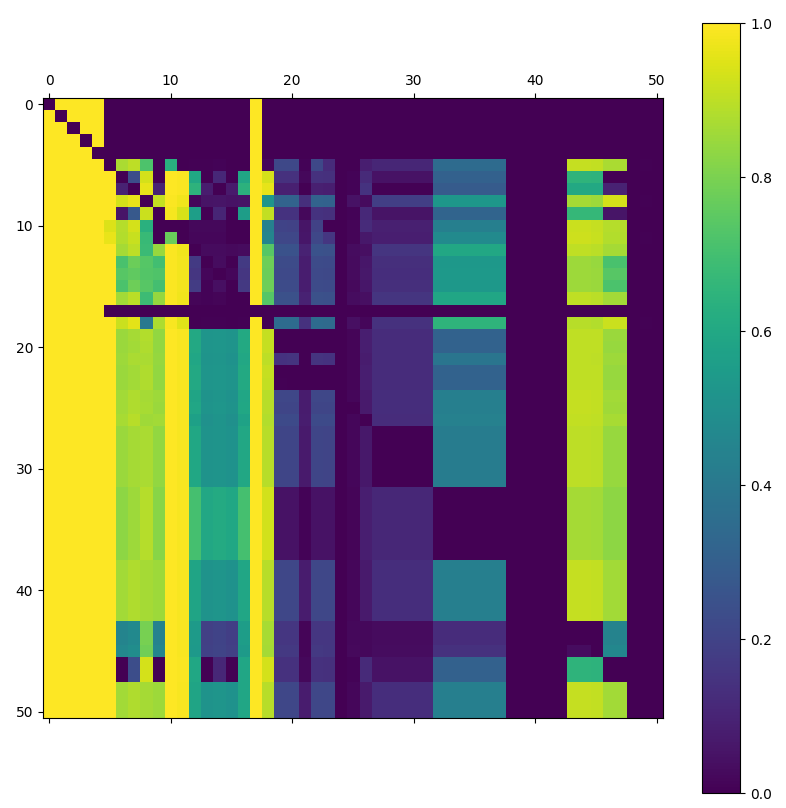
\includegraphics[scale=0.4]{thesis_res/cond/heatmap_cropped.png}
          \caption{Conditional probabilities matrix showing each element's (i,j) probability that feature j is not missing when feature i is missing}
          \label{figure:cond_prob_matrix}
        \end{figure}
        \newpage
      \subsubsection{Feature substitution}
        \noindent Combining the conditional probabilities matrix with the correlation matrix, it is possible to set a correlation threshold and pick only those pairs of features that are correlated above that threshold. With this list of pairs it is then possible to look at the conditional probabilities matrix and see how often is one of the features not missing when the other one is. That way, an algorithm like the surrogate splits \cite{splits} could take these highly correlated pairs into account. If there were a feature that is missing everytime another feature is not missing, the algorithm could base the decision on the value of the other feature.
        \\~\\
        \noindent In other words, let us for example say that feature A is highly correlated with feature B. Feature A is missing 70\% of times while feature B is missing only 20\% of the time. Since they are highly correlated, the classifier can base its decision on feature B instead of on feature A when feature A is missing. The next part of this analysis looks at each feature and studies how many different features can be used in the classification instead of them when they are missing.
        \\~\\
        \noindent Setting the correlation thresholds to 0.3, 0.5 and 0.8 showed that a small amount of features have some correlated features that could substitute for them. With the threshold set to 0.3, there are 20 features that have at least one candidate. [\ref{figure:corr_03}][\ref{figure:corr_05}][\ref{figure:corr_08}] The figures show each feature and the number of their correlated counterparts. This count of correlated features depends on the conditional probability of them being not missing when the feature they are correlated to is missing. The numbers on the y axis are the conditional probability thresholds. As expected, when this threshold increases, the amount of correlated features decreases.
        \newpage
        \noindent In Figure [\ref{figure:corr_03}] it is possible to see that the most prominent features are features 13, 14 and 15. When they are missing, there is at least a 10\% probability that 9 other features are present that could take their place. As the required probability increases, up until 60\% there are 6 of those features.
        \begin{figure}
          \centering
          \includegraphics[scale=0.5]{thesis_res/corr_03_cropped.png}
          \caption{Counts of potential substitions based on their non-missingness probability for each feature with correlation threshold 0.3}
          \label{figure:corr_03}
        \end{figure}
        \newpage
        \noindent Figure [\ref{figure:corr_05}] shows that with correlation threshold set to 0.5, only 8 relevant features remain, with the maximum of 4 correlated features for feature 20. The probability threshold is also much lower than in the previous case.
        \begin{figure}
          \centering
          \includegraphics[scale=0.5]{thesis_res/corr_05_cropped.png}
          \caption{Counts of potential substitions based on their non-missingness probability for each feature with correlation threshold 0.5}
          \label{figure:corr_05}
        \end{figure}
        \newpage
        \noindent Correlation threshold of 0.8 further reduces the number of relevant features to 6 [\ref{figure:corr_08}]. The maximum of correlated features in this case is only 2.
        \begin{figure}
          \centering
          \includegraphics[scale=0.5]{thesis_res/corr_08_cropped.png}
          \caption{Counts of potential substitions based on their non-missingness probability for each feature with correlation threshold 0.8}
          \label{figure:corr_08}
        \end{figure}
        \\~\\
        \noindent A conclusion can be made, that although there are some features that can be substituted by other features when they are missing, the probability of the substitution features not being missing is not very high. Also, as the demand for correlation between these features increases, the amount of potential candidates decreases rapidly.
  \newpage
  \section{Handling missing values}
    In statistics, {\it missing values} or {\it missing data} mark the absence of value in a feature variable of an observed sample. Missing data within a dataset make it impossible for conventional machine learning algorithms to properly learn from it. Many of these algorithms require complete data and do not have an implicit way of handling missing values. In order for the statistical analysis to work, the missing data have to be somehow dealt with beforehand. \cite{otfi}
    \\~\\
    There are various ways of handling missing data, some as simple as dropping the samples containing any missing values altogether, leaving only those samples with all data present. \cite{lwd} This however, cannot be done when there are missing data somewhere in most of the observations. Another simple method, the strawman imputation \cite{otfi} would be replacing missing data with the mean or median of all the non-missing values of the feature in question. The process of replacing the missing data is called {\it imputation}. Only the imputation methods related to random forests are examined in this thesis because of the nature of the analysed data. Also, most of the interesting imputation methods already are in this subset.
    \\~\\
    More sophisticated methods of imputation also exist and they are discussed more thoroughly in this thesis. Some methods work better with smaller datasets, or with datasets with low missingness ratio. The amount of correlation between feature variables can also be important to some methods and not that important to others. \cite{otfi} Some imputation algorithms are very slow and using them in experiments with big datasets can get seriously time-consuming. In other words, choosing a relevant method of imputation for a given dataset is not a simple task and it can prove useful to do an analysis of the data as well as an analysis of the imputation algorithm itself beforehand.
    \subsection{Related work}
      Various works comparing different imputation methods were published in the last years. Multiple imputation methods meant for decision trees are well explained in \cite{mia}.
      \\~\\
      Another work worth mentioning that focuses on random forests and missing data imputation is \cite{rsf}. It introduces a new type of random forests along with the {\it adaptive tree imputation} method. However, this method can be used with regular random forests as well.
      \\~\\
      Perhaps the most recent work on this topic is \cite{otfi} which is a continuation of the previous work by one of the same authors. In this paper, multiple approaches to imputation using random forests are discussed in detail and tested on multiple datasets with different attributes. A comparison of their imputation accuracy is made as well. The datasets used in this work are both real and synthetic. However, the missingness is induced manually \cite{otfi} and thus the results of the experiments can be biased.
    \\~\\
    \subsection{Missing data mechanisms}
      \label{sec:missmech}
      Missing data are usually divided into three categories, depending on the characteristics of their missingness. These categories are also called missing data mechanisms. \cite{lwd} It is important to understand these mechanisms in order to make an educated assumption about the dataset in question. If an assumption is made that the values are missing completely at random while they are missing systematically, an analysis based on this assumption may be biased.
      \begin{itemize}
      \item If the samples with missing data are a random subset of all observed samples, they have a similar distribution. There is no relationship between whether a value is missing and any other value in the data set, be it missing or observed. These values are {\it missing completely at random} (MCAR). \cite{lwd} When a dataset has missing values that are MCAR, it can still be analysed with unbiased results, provided that there are enough observed samples. However, data that are truly MCAR are not encountered often.
      \item When the missing data is somehow dependent or related to other non-missing values in the observation, the data is {\it missing at random} (MAR). \cite{lwd} There is no definitive way of distinguishing between MCAR and MAR data. The assumption of it being one or the other is only as good as the knowledge of the data and the field of the one proposing the assumption. A good example of MAR data would be that males are less likely to fill a depression survey, although it does not have any connection to their level of depression.
      \item The last missing data mechanism is {\it missing not at random} (MNAR). It means that there is a relationship between value of the variable that is missing and the reason why it is missing in the first place. For example a male suffering from a strong depression can decide not to fill a depression survey because of said depression.
      \end{itemize}
    \subsection{Selected imputation algorithms}
      This section contains a list of imputation algorithms that were taken in consideration when deciding which ones to implement.
      \subsubsection{Baseline imputation}
        \label{sec:baseline}
        This method will be used throughout the thesis as the baseline reference value. It replaces the missing data with a constant value outside of the features' interval before growing the tree. Thus, when an object is evaluated and the relevant feature is missing, the object is always sent either to the left or to the right, based on the value that was chosen at the start.
      \subsubsection{Strawman imputation}
        \label{sec:strawman}
        {\it Strawman imputation} \cite{otfi} is a simple method for handling missing values. It works very fast compared to other methods and its implementation is very simple. The missing values are imputed before the forest is grown by calculating the median of non-missing values in the feature column. An altered variation of strawman imputation uses the mean instead of the median.
      \subsubsection{On-the-fly-imputation}
        \label{sec:otfi}
        {\it Adaptive tree imputation} \cite{rsf} later named as {\it On-the-fly-imputation} \cite{otfi} (OTFI) is a method of imputing missing data at the time of growing the tree. That is also where its name comes from. It draws a random value from the non-missing in-bag dataset within the current node to impute the missing values. The algorithm works as follows: 
        \begin{enumerate}
        \item First, the best split is calculated as usual, using only non-missing data.
        \item After finding the best split, random values from the non-missing in-bag data within the current node are used to impute the missing values.
        \item Once the data are imputed, the node is split into the left and right children nodes and the imputed data are reset back to missing.
        \end{enumerate}
        The values the algorithm uses to impute the missing data are stored within the decision node while growing the tree along with the respective frequencies in which they occur within the node's dataset. These are then used again to impute the missing values in the testing dataset at the time of prediction to decide whether the observation belongs to the left or to the right child. After being sent to the child node, the imputed data is reset to missing again and the process repeats.
        \\~\\
        The implementation of OTFI algorithm used for experiments in this thesis had to be improved in order to increase imputation speed and reduce the memory used. Instead of storing the non-missing values and their frequencies, only the probability of the node going left or right is saved at the node. That way, when a new object with a missing value at the relevant feature is examined, the missing value is not imputed at all.
      \subsubsection{Missingness incorporated in attributes}
        \label{sec:mia}
        {\it Missingness incorporated in attributes} \cite{mia} (MIA) works similarly to OTFI in that it also imputes missing data during the forest growing process. It searches for the best split in three different approaches to the missing data. Let {\it X} be a numeric feature used to split a node and {\it s} a possible split value of {\it X}. Over all split values, the method looks at the following:
        \begin{itemize}
        \item Split A: \{ $X \leq s$ or $X =$ missing \} versus \{ $X > s$ \}.
        \item Split B: \{ $X \leq s$ \} versus \{ $X > s$ or $X =$ missing \}.
        \item Split C: \{ $X =$ missing \} versus \{ $X =$ not missing \}.
        \end{itemize}
        After finding the best split in each approach separately, the algorithm then chooses which one of them provides a better information gain and then it splits the dataset accordingly. As in the OTFI method, the MIA implementation used in this thesis makes the decision node remember which split type it had used in order to decide how the testing data should be propagated during prediction.
        \\~\\
        This algorithm is in practice an extension of the method that was used as a baseline. The baseline in fact does the same thing as split A in here. It follows that this method takes approximately three times more time than the baseline.
      \subsubsection{Other algorithms}
        Other notable imputation algorithms were also considered, such as {\it surrogate splits} \cite{splits} or {\it missForest} \cite{otfi}. However, surrogate splits perform less reliably as the amount of missing data increases \cite{splits} and are slow when used with larger datasets. \cite{rsf} The low computational speed is a problem for missForest as well, making it "100's of times" slower than methods like OTFI or MIA. \cite{otfi} Since the network traffic dataset is very big and a big portion of its data is missing [\ref{sec:datadesc}], these methods are not very relevant and they are not in the scope of this thesis.
  \newpage
  \section{Experiments}
    \label{sec:experiments}
    This chapter focuses on the experiments done with network data regarding the performance of several imputation methods. The first part describes the measures used for evaluation and why they were used. The second part looks at the results of the experiments and their comparison. All of the experiments were done on the same data, that is the network traffic logged on three days of January 2017, each of them a week after the previous one, was used as the training dataset, whereas the testing dataset was a single day of March of the same year. Each experiment was evaluated in three different ways - {\it unaggregated}, {\it aggregated}, and {\it aggregated relaxed}. Unaggregated means that the performance is evaluated in a regular per-row manner. Aggregated (by one of the metadata column, for example a user) evaluation is done in order to remove duplicities (multiple records marking the same user as a suspect of malware infection) and removes negative records if there is at least one positive one. This makes sense because if a user is infected, the network traffic he produces can be either regular or point to some malware infection. This aggregation removes the arguably unimportant, clean data. It is done to reflect the seen performance by the customers who are not interested in flows, but in users. Going a level further, the aggregated relaxed evaluation clears the differences between different classes of malware and reduces the classification problem into the binary case - infected, or not infected. Yet the classifier itself still remains multiclass.
    \subsection{Evaluation metrics}
      There is a plenty of measures that can be used to determine the classifier's performance. The most commonly observed is perhaps the {\it classification error} \cite{brabec}. The problem with classification error is that it does not say much when the dataset is imbalanced, as is the situation with the network data. For example if we had a dataset where there are 10,000 samples and only 1 of them belonged to a positive class, the classifier could classify all samples as negative and it would achieve a classification error of 0.01\%. In this project we are interested in two different measures, {\it precision} and {\it recall}. In order to compute them, we also need the {\it confusion matrix}.
      \subsubsection{Confusion matrix}
        In binary classification, we can label the two classes as positive and negative. {\it Confusion matrix} \cite{confusion} divides the classification results into the following categories:
        \begin{description}
        \item [TP:]   True positives. The number of positive objects the classifier labeled as positive.
        \item [FP:]   False positives. The number of negative objects the classifier labeled as positive.
        \item [TN:]   True negatives. The number of negative objects the classifier labeled as negative.
        \item [FN:]   False negatives. The number of positive objects the classifier labeled as negative.
        \end{description}
        These categories are then used to compute other, more interesting measures.
        \\~\\
        In multiclass classification, the {\it confusion matrix} gets more complicated. Consider a dataset with 3 different classes A, B and C. If the classifier takes a sample that belongs to class A and labels it as B, then it counts as FN for class A, but as FP for class B.
        \\~\\
        This gets even more confusing with the network datasets. The samples are either negative and thus belonging to one specific class, or positive, which means one of multiple positive classes. For that reason, samples belonging to the negative classes that are classified as negative do not count as TP. Similarly, when a positive sample is labeled as positive but a different class, it should not be counted as FN, rather as TPish. As for TNs, it does not make much sense to distinguish them from TPs, since they basically are TPs for the negative class. This is a way of reducing the multiclass problem to a binary problem. In the context of this project, a {\it one-vs-all} confusion matrix, which evaluates one class at a time, is computed. Furthermore, TNs do not get counted and the TPs of the negative class are optionally filtered out in the process.
      \subsubsection{Precision}
        {\it Precision}, or {\it positive predictive value} \cite{confusion} is defined as:
        \begin{equation}
          Precision = \frac{TP}{TP + FP}
        \end{equation}
        Precision is the fraction of positive objects among all objects that the classifier labeled as positive. It can also be interpreted as the probability that a positively labeled object is truly positive. A precision score of 1.0 means that every object labeled as positive by the classifier is truly positive. It does not say, however, anything about the classifier's ability to recognize all truly positive instances. In multiclass environment, precision of every class varies because it is computed separately.
      \subsubsection{Recall}
        {\it Recall}, or {\it sensitivity} \cite{confusion} is defined as:
        \begin{equation}
          Recall = \frac{TP}{TP + FN}
        \end{equation}
        Recall is the fraction of positive objects that the classifier labeled as positive among all truly positive objects. It can be interpreted as the probability that a truly positive object is labeled as positive. A recall score of 1.0 means that every truly positive object is labeled as positive by the classifier. This could be achieved simply by labeling all objects as positive, recall does not say anything about the number of false positives. Recall of every class varies among all classes in multiclass environment.
    \\~\\
    For a better comprehension of precision and recall, Figure [\ref{figure:precrec}] shows what they represent.
    \begin{figure}
      \centering
      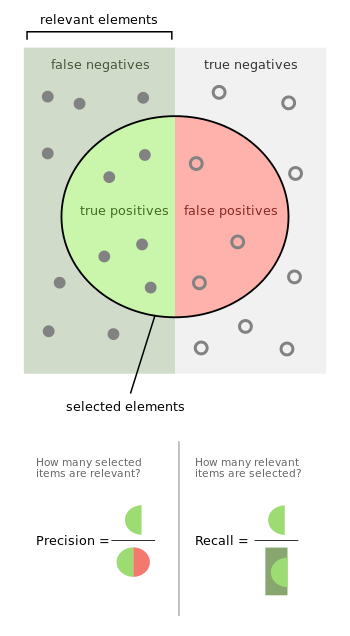
\includegraphics[scale=0.8]{thesis_res/precrec.png}
      \caption{Visual representation of precision and recall \cite{precrec}}
      \label{figure:precrec}
    \end{figure}
    \newpage
    \subsection{Results}
      This subsection presents the results of the individual experiments. The main focus is the average prediction precision, recall and also the number of classes that were predicted with precision above specific thresholds. The following tables will always show all three evaluation approaches (unaggregated, aggregated, relaxed) for every tested method. The tested methods are the baseline [\ref{sec:baseline}] method, the Strawman [\ref{sec:strawman}] imputation method both with mean and median values, the OTFI [\ref{sec:otfi}] method and the MIA [\ref{sec:mia}] method. The two variations of the Strawman method are further referred to simply as mean and median.
      \\~\\
      The randomness factor of random forests gives the resulting precision and recall a variance of about 1\%. So if one method has a precision of 10\% and another one only 8\%, we can assume that their performance could be the same.
      \subsubsection{Average overall precision}
        The first metric to look at is the overall precision averaged across all classes. However, in this case only the positive classes are relevant, so the negative class is excluded. Looking at Figure [\ref{figure:overall_prec}], it can be seen that the OTFI method does not bring any improvement compared to the baseline and its results are actually even weaker. This could be happening because the OTFI method computes the split statistic from the not missing data and therefore does not have enough data to grow the trees sufficiently. The MIA method performs slightly better than the baseline while the Strawman imputation using mean value performs equally. The Strawman using median proved to be worse.
        \begin{figure}
          \centering
          \caption{Precision of the tested methods averaged across all positive classes}
          \label{figure:overall_prec}
          \begin{tikzpicture}
            \begin{axis}[
                ybar,
                width=12cm,
                height=10cm,
                symbolic x coords={Baseline, Mean, Median, Otfi, Mia},
                xtick=data,
                legend style={at={(0.5, -0.2)},
                  anchor=north,legend columns=-1},
                x tick label style={
                  rotate=90,
                  anchor=east,
                },
            ]
              \addplot coordinates {
                (Baseline, 0.6100512556192825) (Mean, 0.5929441385687005) (Median, 0.5559723904131693) (Otfi, 0.23076311507408218) (Mia, 0.6474093791131115)
              };
              \addplot coordinates {
                (Baseline, 0.5174926507483615) (Mean, 0.5099029457463545) (Median, 0.46407370725945946) (Otfi, 0.20295490146464956) (Mia, 0.561308648654571)
              };
              \addplot coordinates {
                (Baseline, 0.5347665149666363) (Mean, 0.53004735287115) (Median, 0.46687743259161074) (Otfi, 0.2033114832567041) (Mia, 0.5763728141572483)
              };
              \legend{Unaggregated, Aggregated, Relaxed}
            \end{axis}
          \end{tikzpicture}
        \end{figure}
      \newpage
      \subsubsection{Number of classes with precision above a certain threshold}
        Average overall precision works as a metric to give a solid first view of the classifier's performance. However, it does not say much about the balance of the classifier. If the testing dataset had for example 90 objects of class 1 and the remaining 10 objects were of 10 different classes, the average overall precision could be 0.9. Sadly, that does not say if the classifier recognized all the classes, or only the one with 90 samples.
        \\~\\
        Because of that, it is good to look at the number of classes that were predicted with precision above some chosen threshold. The thresholds chosen for this experiment are 0.5, 0.8, 0.9, 0.95 and 1.00. Table [\ref{table:prec_above}] shows the number of classes with precision above these threshold for each method and each evaluation aproach along with the average recall of the classes in question underneath them.


\begin{table}[]
\centering
\caption{The number of classes predicted with precision above a specified threshold \newline}
\label{table:prec_above}
\resizebox{\columnwidth}{!}{%
\begin{tabular}{|
>{\columncolor[HTML]{ECF4FF}}l |c|c|c|c|c|c|c|c|c|c|c|c|c|c|c|}
\hline
\multicolumn{1}{|c|}{\cellcolor[HTML]{ECF4FF}\begin{tabular}[c]{@{}c@{}}Method\\ U / A / R\end{tabular}} & \multicolumn{3}{c|}{\cellcolor[HTML]{ECF4FF}Baseline}                                                                                                        & \multicolumn{3}{c|}{\cellcolor[HTML]{ECF4FF}Mean}                                                                                                            & \multicolumn{3}{c|}{\cellcolor[HTML]{ECF4FF}Median}                                                                                                          & \multicolumn{3}{c|}{\cellcolor[HTML]{ECF4FF}OTFI}                                                                                                            & \multicolumn{3}{c|}{\cellcolor[HTML]{ECF4FF}MIA}                                                                                                             \\ \hline
\begin{tabular}[c]{@{}l@{}}\# of classes\\ prec \textgreater { }0.5\\ avg recall \%\end{tabular}            & \begin{tabular}[c]{@{}c@{}}70\\ \\ 74\end{tabular} & \begin{tabular}[c]{@{}c@{}}61\\ \\ 83\end{tabular} & \begin{tabular}[c]{@{}c@{}}63\\ \\ 84\end{tabular} & \begin{tabular}[c]{@{}c@{}}70\\ \\ 76\end{tabular} & \begin{tabular}[c]{@{}c@{}}59\\ \\ 82\end{tabular} & \begin{tabular}[c]{@{}c@{}}63\\ \\ 82\end{tabular} & \begin{tabular}[c]{@{}c@{}}65\\ \\ 70\end{tabular} & \begin{tabular}[c]{@{}c@{}}52\\ \\ 80\end{tabular} & \begin{tabular}[c]{@{}c@{}}52\\ \\ 80\end{tabular} & \begin{tabular}[c]{@{}c@{}}25\\ \\ 27\end{tabular} & \begin{tabular}[c]{@{}c@{}}22\\ \\ 25\end{tabular} & \begin{tabular}[c]{@{}c@{}}22\\ \\ 25\end{tabular} & \begin{tabular}[c]{@{}c@{}}74\\ \\ 74\end{tabular} & \begin{tabular}[c]{@{}c@{}}67\\ \\ 85\end{tabular} & \begin{tabular}[c]{@{}c@{}}68\\ \\ 85\end{tabular} \\ \hline
\begin{tabular}[c]{@{}l@{}}\# of classes\\ prec \textgreater { }0.8\\ avg recall \%\end{tabular}            & \begin{tabular}[c]{@{}c@{}}54\\ \\ 74\end{tabular} & \begin{tabular}[c]{@{}c@{}}37\\ \\ 87\end{tabular} & \begin{tabular}[c]{@{}c@{}}39\\ \\ 88\end{tabular} & \begin{tabular}[c]{@{}c@{}}54\\ \\ 77\end{tabular} & \begin{tabular}[c]{@{}c@{}}38\\ \\ 87\end{tabular} & \begin{tabular}[c]{@{}c@{}}41\\ \\ 87\end{tabular} & \begin{tabular}[c]{@{}c@{}}45\\ \\ 71\end{tabular} & \begin{tabular}[c]{@{}c@{}}32\\ \\ 85\end{tabular} & \begin{tabular}[c]{@{}c@{}}32\\ \\ 85\end{tabular} & \begin{tabular}[c]{@{}c@{}}25\\ \\ 27\end{tabular} & \begin{tabular}[c]{@{}c@{}}21\\ \\ 26\end{tabular} & \begin{tabular}[c]{@{}c@{}}21\\ \\ 26\end{tabular} & \begin{tabular}[c]{@{}c@{}}60\\ \\ 74\end{tabular} & \begin{tabular}[c]{@{}c@{}}40\\ \\ 86\end{tabular} & \begin{tabular}[c]{@{}c@{}}41\\ \\ 86\end{tabular} \\ \hline
\begin{tabular}[c]{@{}l@{}}\# of classes\\ prec \textgreater { }0.9\\ avg recall \%\end{tabular}            & \begin{tabular}[c]{@{}c@{}}44\\ \\ 73\end{tabular} & \begin{tabular}[c]{@{}c@{}}28\\ \\ 86\end{tabular} & \begin{tabular}[c]{@{}c@{}}31\\ \\ 87\end{tabular} & \begin{tabular}[c]{@{}c@{}}48\\ \\ 78\end{tabular} & \begin{tabular}[c]{@{}c@{}}31\\ \\ 85\end{tabular} & \begin{tabular}[c]{@{}c@{}}33\\ \\ 86\end{tabular} & \begin{tabular}[c]{@{}c@{}}39\\ \\ 71\end{tabular} & \begin{tabular}[c]{@{}c@{}}26\\ \\ 84\end{tabular} & \begin{tabular}[c]{@{}c@{}}26\\ \\ 84\end{tabular} & \begin{tabular}[c]{@{}c@{}}25\\ \\ 27\end{tabular} & \begin{tabular}[c]{@{}c@{}}19\\ \\ 25\end{tabular} & \begin{tabular}[c]{@{}c@{}}19\\ \\ 25\end{tabular} & \begin{tabular}[c]{@{}c@{}}53\\ \\ 74\end{tabular} & \begin{tabular}[c]{@{}c@{}}34\\ \\ 86\end{tabular} & \begin{tabular}[c]{@{}c@{}}35\\ \\ 86\end{tabular} \\ \hline
\begin{tabular}[c]{@{}l@{}}\# of classes\\ prec \textgreater { }0.95\\ avg recall \%\end{tabular}           & \begin{tabular}[c]{@{}c@{}}37\\ \\ 71\end{tabular} & \begin{tabular}[c]{@{}c@{}}25\\ \\ 85\end{tabular} & \begin{tabular}[c]{@{}c@{}}29\\ \\ 86\end{tabular} & \begin{tabular}[c]{@{}c@{}}38\\ \\ 75\end{tabular} & \begin{tabular}[c]{@{}c@{}}26\\ \\ 84\end{tabular} & \begin{tabular}[c]{@{}c@{}}28\\ \\ 85\end{tabular} & \begin{tabular}[c]{@{}c@{}}36\\ \\ 70\end{tabular} & \begin{tabular}[c]{@{}c@{}}23\\ \\ 83\end{tabular} & \begin{tabular}[c]{@{}c@{}}23\\ \\ 83\end{tabular} & \begin{tabular}[c]{@{}c@{}}24\\ \\ 26\end{tabular} & \begin{tabular}[c]{@{}c@{}}19\\ \\ 25\end{tabular} & \begin{tabular}[c]{@{}c@{}}19\\ \\ 25\end{tabular} & \begin{tabular}[c]{@{}c@{}}45\\ \\ 71\end{tabular} & \begin{tabular}[c]{@{}c@{}}33\\ \\ 87\end{tabular} & \begin{tabular}[c]{@{}c@{}}35\\ \\ 86\end{tabular} \\ \hline
\begin{tabular}[c]{@{}l@{}}\# of classes\\ prec = 1.00\\ avg recall \%\end{tabular}                      & \begin{tabular}[c]{@{}c@{}}22\\ \\ 56\end{tabular} & \begin{tabular}[c]{@{}c@{}}22\\ \\ 83\end{tabular} & \begin{tabular}[c]{@{}c@{}}27\\ \\ 85\end{tabular} & \begin{tabular}[c]{@{}c@{}}21\\ \\ 63\end{tabular} & \begin{tabular}[c]{@{}c@{}}23\\ \\ 83\end{tabular} & \begin{tabular}[c]{@{}c@{}}26\\ \\ 84\end{tabular} & \begin{tabular}[c]{@{}c@{}}19\\ \\ 57\end{tabular} & \begin{tabular}[c]{@{}c@{}}20\\ \\ 81\end{tabular} & \begin{tabular}[c]{@{}c@{}}20\\ \\ 81\end{tabular} & \begin{tabular}[c]{@{}c@{}}18\\ \\ 16\end{tabular} & \begin{tabular}[c]{@{}c@{}}18\\ \\ 26\end{tabular} & \begin{tabular}[c]{@{}c@{}}18\\ \\ 26\end{tabular} & \begin{tabular}[c]{@{}c@{}}28\\ \\ 62\end{tabular} & \begin{tabular}[c]{@{}c@{}}28\\ \\ 85\end{tabular} & \begin{tabular}[c]{@{}c@{}}31\\ \\ 86\end{tabular} \\ \hline
\end{tabular}}
\end{table}























      \subsubsection{Average overall recall}
        Apart from precision, the second studied measure was recall. As with the precision, the recall is averaged across all classes except for the negative one. OTFI method's very small recall again shows how ineffective the method is when it is used on the network data. [\ref{figure:overall_recall}]
        \begin{figure}
          \centering
          \caption{Recall of the tested methods averaged across all positive classes}
          \label{figure:overall_recall}
          \begin{tikzpicture}
            \begin{axis}[
                ybar,
                width=12cm,
                height=10cm,
                symbolic x coords={Baseline, Mean, Median, Otfi, Mia},
                xtick=data,
                legend style={at={(0.5, -0.2)},
                  anchor=north,legend columns=-1},
                x tick label style={
                  rotate=90,
                  anchor=east,
                },
            ]
              \addplot coordinates {
                (Baseline, 0.5711167103861942) (Mean, 0.5409939453125392) (Median, 0.4917962171048626) (Otfi, 0.0621788730236572) (Mia, 0.5842264543107969)
              };
              \addplot coordinates {
                (Baseline, 0.6517120595074839) (Mean, 0.6107092982021902) (Median, 0.5762881167127762) (Otfi, 0.06707380091104026) (Mia, 0.6661638824968948)
              };
              \addplot coordinates {
                (Baseline, 0.6625921022559819) (Mean, 0.6238587519352431) (Median, 0.5780854570007973) (Otfi, 0.06714536161898142) (Mia, 0.6774127175483475)
              };
              \legend{Unaggregated, Aggregated, Relaxed}
            \end{axis}
          \end{tikzpicture}
        \end{figure}
        \newpage
        From the results it can be clearly seen that the Strawman imputation, both with the mean value or the median value, work similar to the baseline imputation, if not a little worse. As could have been expected, the MIA imputation method on the other hand works a little better than the baseline method, which is because it contains the baseline in its own implementation, and then looks a little longer to see if it can find a better split. The OTFI method, however, did not work so well. The reason for that is that the network dataset has more than a half [\ref{sec:analysis}] of its values missing and the algorithm only uses the data that is not missing when finding the best split.
  \newpage
  \section*{Conclusion}
  \addcontentsline{toc}{section}{Conclusion}
    The focus of this thesis was to examine the problem of handling missing values in network traffic datasets. The thesis introduced a number of existing methods for imputation of missing data, but not all of them are relevant to the network datasets. Most of the algorithms do not scale well with bigger amounts of data missing or they run very slow on big datasets, so only the relevant were implemented.
    \\~\\
    The implemented methods were tested and compared, showing that the MIA imputation method provides a slight improvement in both prediction precision and prediction recall over the method used as the baseline. While the baseline's unaggregated averaged precision was 61\%, the MIA method's averaged precision was about 65\%. In the aggregated approach, baseline's score is 52\% and MIA's 56\%. The relaxed precision is 53\% for the baseline and 58\% for MIA. As for recall, baseline's average is 57\% unaggregated, 65\% aggregated and 66\% relaxed, while MIA scored about one percent higher with 58\% unaggregated, 66\% aggregated and 68\% relaxed.
    \\~\\
    The OTFI method on the other hand provided much worse results than the baseline, showing that it also belongs to the methods that do not scale well with heavy missingness because it uses only the non-missing data in computing the split statistics.
    \\~\\
    The Strawman imputation method ended up close to the baseline, but did not surpass it. The Strawman variation using mean of the features as the imputation provided better results than the median variation.
    \\~\\
    Apart from that, an analysis on the dataset was done to find the correlations between the features' values and their missingness. Some of the features proved to be missing exclusively together, but not all of them. Some features' values are significantly correlated and in some cases it was found out that when one the features is missing, then its correlated pair has a reasonable probability of being not missing. This can be used in the future to further enhance the classifier's performance.
  \newpage
  \bibliography{thesis}
  \addcontentsline{toc}{section}{Reference}
  \newpage
  \appendix
    \section{Enclosed CD contents}
      The root directory on the enclosed CD contains the following items:
      \begin{description}
        \item[thesis.pdf:] The PDF file with the thesis.
        \item[src:] The source directory with all implemented code written in Python.
      \end{description}
\end{document}

